\section{Discussão}

\subsection{Modelagem matemática de uma esfera carregada sob o campo do Van der Graaff}
Conforme discutido anteriormente, duas cargas iguais exercem uma força de repulsão entre si. Podemos, então extrapolar este resultado para modelar o ângulo formado por uma esfera carregada com carga de mesmo sinal pendurada por um fio isolante há uma distância \(r\) do centro do van de Graaff. Tal experimento está ilustrado na \cref{vander}

\begin{figure}[htb]
    \centering
    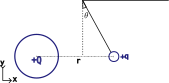
\includegraphics[width=.5\linewidth]{figs/vanderball.png}
    \caption{esfera carregada a uma distância \(r\) do van der Graaff igualmente carregado pendurada por um fio isolante e formando um ângulo \(\theta\) com a vertical usualmente formada na ausência do campo elétrico}\label{vander}
\end{figure}

\begin{align*}
    {|T|} &= \frac{{|P|}}{\cos \theta}\\
    {|T|} &= \frac{{|F_{e}|}}{\sin \theta}\\
    \implies \frac{{|P|}}{\cos \theta} &= \frac{{|F_{e}|}}{\sin \theta}\\
    \implies \theta &= \arctan \left( \frac{{|F_{e}|}}{{|P|}}\right) 
\end{align*}

Podemos utilizar a lei de Coulomb para determinar a força elétrica em função da carga \(Q\) do van der Graaff:
\begin{align*}
    F_{e} = \frac{qQ}{4 \pi \varepsilon_{0} r^{2}}
\end{align*}

Assim, substituindo na fórmula:
\begin{align*}
    \theta &= \arctan \left( \frac{qQ}{4 \pi \varepsilon_{0}r^{2}{mg}} \right)
\end{align*}

Com isso, seria possível testar este ângulo como medida indireta da lei de Coulomb. No entanto, não pudemos realizar esta medida pela falta de uma bola e um fio isolante no lab demo.

\subsection{Medida da força elétrica entre canudos}
Para testar a Lei de Coulomb, os dois canudos carregados foram suspensos como pêndulos idênticos (massa \(m\), comprimento da haste/corda \(L\)) de modo a alcançar um equilíbrio estático com deflexão angular \(\theta\). No equilíbrio, a força eletrostática \(F\) é balanceada pela componente horizontal da tensão no fio, levando às relações
\begin{align*}
    T\cos\theta = mg,\qquad T\sin\theta = F_{e}
\end{align*}

logo
\begin{align*}
F_{e} = mg\tan\theta.
\end{align*}

A separação entre cargas foi tomada como \(r=2L\sin\theta\). A Lei de Coulomb foi verificada comparando-se \(F_{e}\) com a expressão

\begin{align*}
F_{e} = k\frac{q_1 q_2}{r^2},
\end{align*}
onde \(k=\dfrac{1}{4\pi\varepsilon_0}\). A partir das medidas experimentais (\(\theta\), \(m\), \(L\) e \(r\)) obteve-se \(F_{e}\) e, quando aplicável, a carga equivalente por

\begin{align*}
q = \sqrt{\dfrac{F_{e}\,r^{2}}{k}} \quad(\text{para } q_1=q_2=q).
\end{align*}

\subsection{Efeito triboelétrico e carregamento do Van de Graaff}
O carregamento do gerador ocorreu por transferência de carga entre materiais em contato/fricção (efeito triboelétrico) e posterior transporte por uma correia isolante. A correia recolhe cargas na região inferior (escova/ pente coletor) e as transporta para a esfera superior, onde outra escova/pente referencia a transferência ao domo, acumulando potencial. O acúmulo adicional é facilitado por descargas coronais controladas através de eletrodos de coleta e isolamento apropriado. No relatório, descreveu-se apenas o mecanismo operacional: fricção → transporte pela correia → deposição no domo por escovas/penas.
